\documentclass[12pt]{article}

%\setlength{\textwidth}{6.4in} \setlength{\textheight}{8.0in}
%\setlength{\oddsidemargin}{.1in} \setlength{\topmargin}{.25in}

\usepackage{amsmath,amssymb,graphicx,multirow,textcomp,color,booktabs}
\usepackage{epsfig,dcolumn,float,rotating}
\usepackage[round]{natbib}
\usepackage[text={7.1in,8in}, top=1.75in, left=0.69in]{geometry}

\bibliographystyle{authordate1}
%\bibliographystyle{plain}

\newcommand{\cp}[1]{\texttt{#1}}
\newcommand{\bibdir}{/bibtex}
%\setcounter{page}{0}
\usepackage{mwe}
\usepackage[export]{adjustbox}
\usepackage{subfig}
\usepackage{chngcntr}
\usepackage{rotating}
\counterwithin{subfigure}{figure}
\DeclareMathSizes{10}{10}{10}{10}
\graphicspath{{figures/}}
\usepackage[absolute]{textpos}
\usepackage{fancyhdr}
\usepackage{lscape}
\fancypagestyle{lscape}{%
\renewcommand{\headrulewidth}{0pt}
\renewcommand{\footrulewidth}{0pt}}

\begin{document}

\title{Web-based Supporting Materials for ``Bayesian quantile regression joint models: inference and dynamic predictions'' by Ming Yang, Sheng Luo and Stacia DeSantis}

\date{}
\maketitle

\setlength{\baselineskip}{23pt}

\section{Distribution comparison}

\begin{figure}[H]
\centering
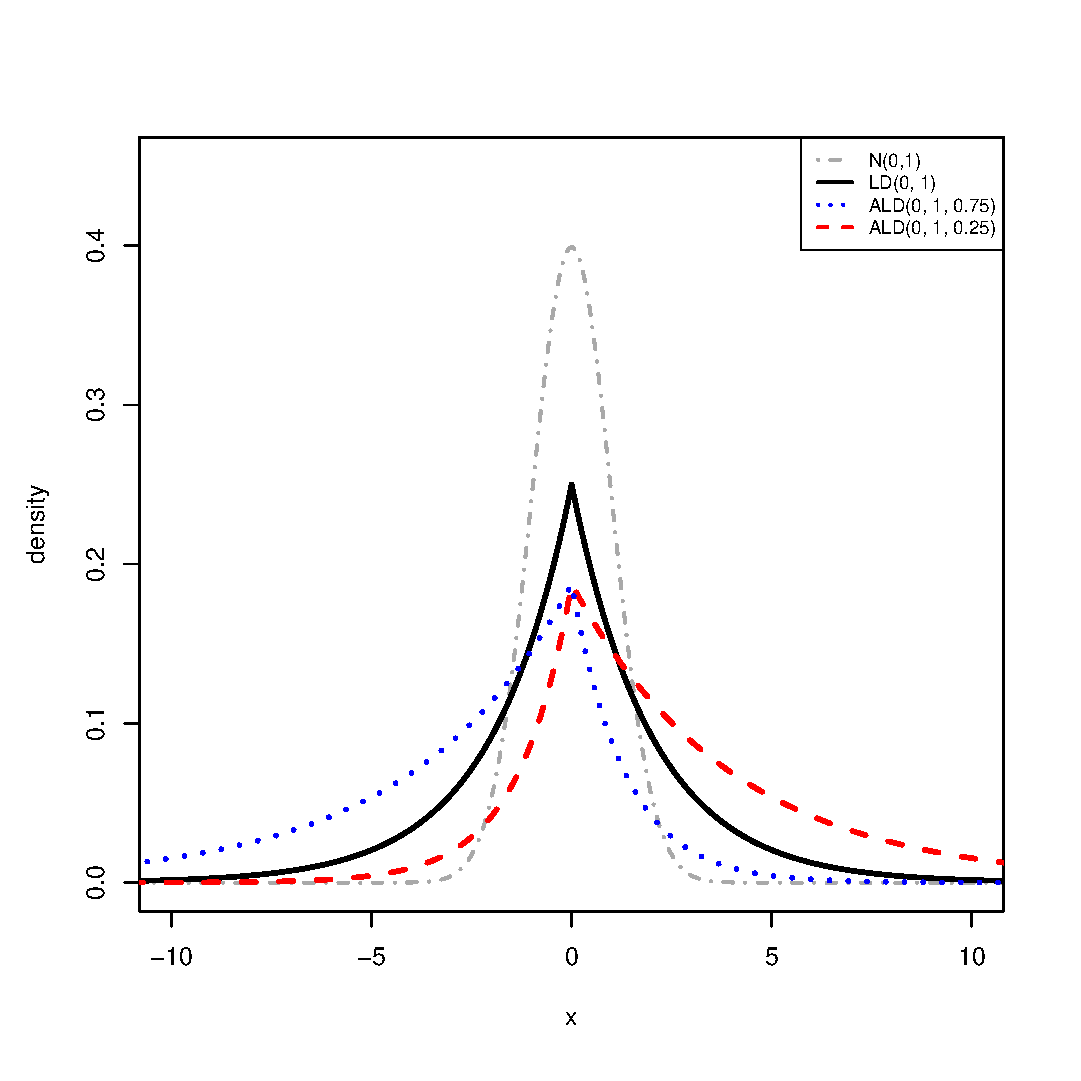
\includegraphics[width=0.4\columnwidth]{figures/ald_ld_normal.eps}\label{plot:ald_ld_normal}
\caption{A comparison of normal, Laplace and asymmetric Laplace distributions.}
\end{figure}

\begin{itemize}
\item Laplace distribution (LD) with location at 0 and scale parameter equals 1 is symmetrical about 0. It has heavier tail compared with standard normal distribution.
\item Asymmetric Laplace distribution (ALD) is either positively or negatively skewed and the direction and degree of skewness are control by the skewness parameter $\tau \in [0,1]$.
\end{itemize}


\newpage
\section{Additional simulation results}\label{sec:appendix_simulation}

\begin{table}[H]
\centering
\caption{Simulation result in Simulation I Scenario 2 in which random errors are generated from ALD with $\tau=0.5$.}
%\adjustbox{max width=\textwidth}{
\label{tab:sim1tab2}
\begin{tabular}{lccccccccc}
\hline
& \multicolumn{4}{c}{QRJM ($\tau=0.5$)} & & \multicolumn{4}{c}{LMJM}\\
\hline
 & Bias & SE & MSE & CP & & Bias & SE & MSE & CP \\
\hline
  \multicolumn{10}{l}{Coefficients for longitudinal process} \\
  $\beta_0$ & $-$0.006 & 0.069 & 0.009 & 0.960 & & 0.013 & 0.093 & 0.017 & 0.960 \\
  $\beta_{1}$ & 0.008 & 0.060 & 0.008 & 0.900 & & 0.018 & 0.079 & 0.018 & 0.880 \\
  $\beta_{2}$ & 0.014 & 0.075 & 0.011 & 0.950 & & 0.031 & 0.093 & 0.021 & 0.940 \\
  \multicolumn{10}{l}{Coefficients for survival process} \\
  $\gamma_1$ & 0.008 & 0.055 & 0.006 & 0.940 & & 0.014 & 0.058 & 0.007 & 0.950 \\
  $\gamma_2$ & 0.007 & 0.055 & 0.007 & 0.950 & & 0.013 & 0.057 & 0.007 & 0.950 \\
  $\alpha$ & $-$0.001 & 0.071 & 0.011 & 0.930 & & $-$0.028 & 0.101 & 0.086 & 0.920 \\
   \hline
\end{tabular}
%}
\end{table}

\begin{table}[H]
\centering
\caption{Simulation result in Simulation I Scenario 3 in which random errors are generated from $N(0, 1)$.}
%\adjustbox{max width=\textwidth}{
\label{tab:sim1tab3}
\begin{tabular}{lccccccccc}
\hline
& \multicolumn{4}{c}{QRJM ($\tau=0.5$)} & & \multicolumn{4}{c}{LMJM} \\
\hline
 & Bias & SE & MSE & CP & & Bias & SE & MSE & CP \\
\hline
  \multicolumn{10}{l}{Coefficients for longitudinal process} \\

  $\beta_0$ & 0.015 & 0.037 & 0.003 & 0.950 & & 0.000 & 0.035 & 0.002 & 0.980 \\
  $\beta_{1}$ & 0.004 & 0.034 & 0.002 & 0.960 & & $-$0.003 & 0.033 & 0.002 & 0.950\\
  $\beta_{2}$ & 0.013 & 0.050 & 0.005 & 0.950 & & 0.006 & 0.049 & 0.005 & 0.950 \\
  \multicolumn{10}{l}{Coefficients for survival process} \\
  $\gamma_1$ & 0.008 & 0.055 & 0.006 & 0.920 & & 0.003 & 0.054 & 0.006 & 0.900 \\
  $\gamma_2$ & 0.015 & 0.055 & 0.007 & 0.920 & & 0.010 & 0.054 & 0.006 & 0.920 \\
  $\alpha$ & $-$0.013 & 0.055 & 0.006 & 0.950 & & 0.007 & 0.055 & 0.006 & 0.950 \\
   \hline
\end{tabular}
%}
\end{table}


\begin{table}[H]
\centering
\caption{Prediction results in Simulation II Scenario 3 in which random errors are generated from $N(0, 1)$.}
%\adjustbox{max width=\textwidth}{
\label{tab:sim2tab2}
\begin{tabular}{clcccccc}
\hline
 & & & \multicolumn{2}{c}{QRJM ($\tau=0.5$)} & &\multicolumn{2}{c}{LMJM}\\
\cline{4-5}\cline{7-8}
$t$ & $\Delta t$ & \multicolumn{1}{p{1.5cm}}{\centering true \\ AUC$_{t}^{\Delta t}$} & $S(t + \Delta t|t)_{MSE}$ & \multicolumn{1}{p{1.5cm}}{\centering predicted \\ AUC$_{t}^{\Delta t}$} & & $S(t + \Delta t|t)_{MSE}$ & \multicolumn{1}{p{1.5cm}}{\centering predicted \\ AUC$_{t}^{\Delta t}$} \\
\hline
\multirow{2}{*}{{\bf 0.25}} & 0.25 & 0.812 & 0.005 & 0.800 && 0.005 & 0.799 \\
&  1 & 0.867 & 0.009 & 0.868 &&  0.009 & 0.869 \\
\multirow{2}{*}{(subjects left: 47.87\%)} &  2 & 0.918 & 0.011 & 0.898 && 0.010 & 0.900 \\
&  3 & 0.936 & 0.011 & 0.916 && 0.011 & 0.917 \\
\hline
\multirow{2}{*}{{\bf 0.5}} & 0.25 & 0.817 & 0.005 & 0.807 && 0.003 & 0.804 \\
& 1 & 0.868 & 0.012 & 0.851 && 0.008 & 0.849 \\
\multirow{2}{*}{(subjects left: 34.78\%)}& 2 & 0.907 & 0.014 & 0.893 && 0.011 & 0.890 \\
&   3 & 0.929 & 0.015 & 0.908 && 0.012 & 0.907 \\
\hline
\multirow{2}{*}{{\bf 0.75}} & 0.25 & 0.807 & 0.008 & 0.801 && 0.002 & 0.787 \\
& 1 & 0.849 & 0.019 & 0.847 && 0.007 & 0.827 \\
\multirow{2}{*}{(subjects left: 27.71\%)} & 2 & 0.892 & 0.021 & 0.890 && 0.011 & 0.876 \\
&  3 & 0.921 &  0.022 & 0.906 && 0.012 & 0.898 \\
\hline
\end{tabular}
%}
\end{table}


\begin{figure}[H]
\centering
\subfloat[][QRJM with $\tau=0.25$ (True model)]{
    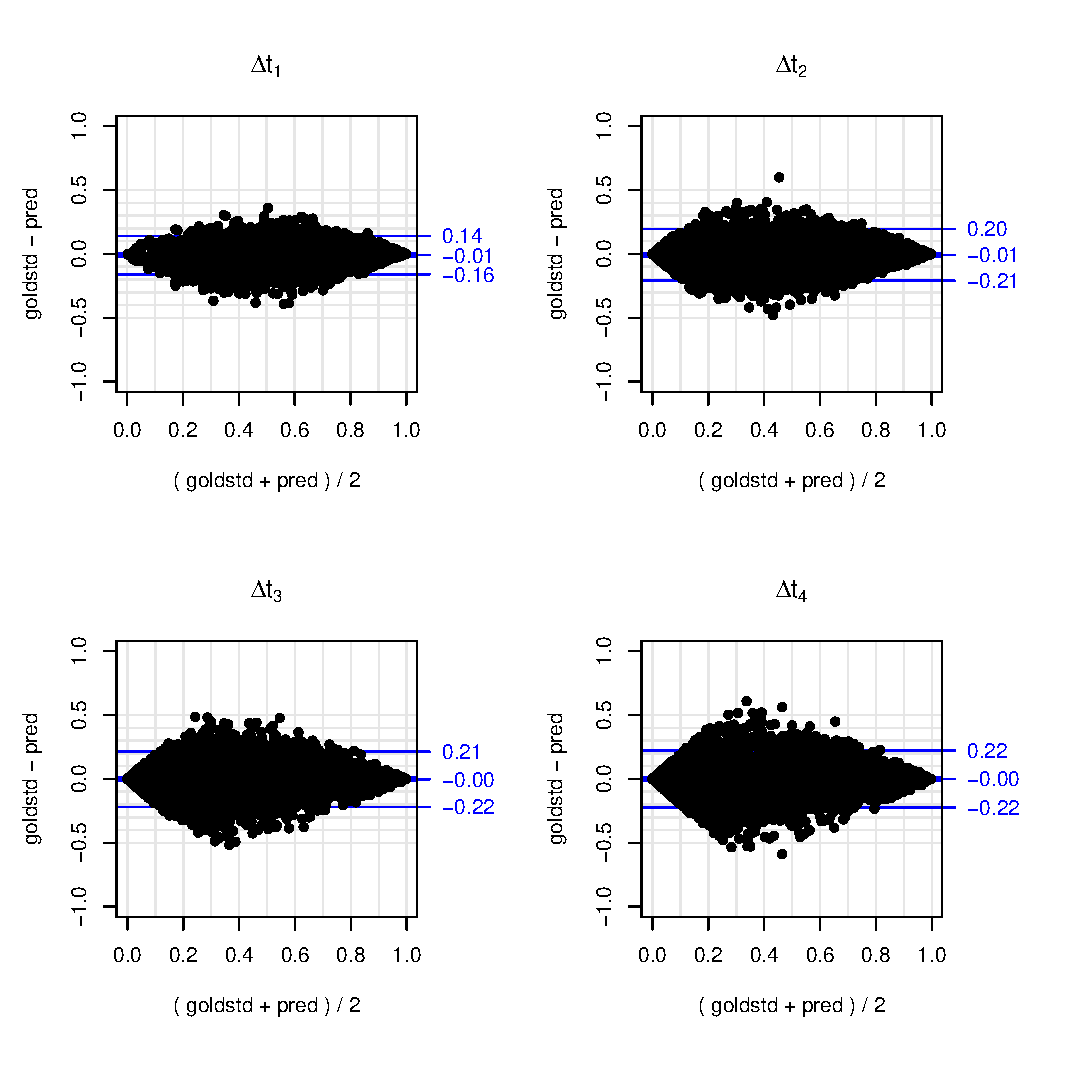
\includegraphics[width=0.45\columnwidth]{figures/baplot_qt25data_qt25fit_t1.eps}\label{plot:sim2fig11}
}
% \centering
\subfloat[][QRJM with $\tau=0.5$]{
    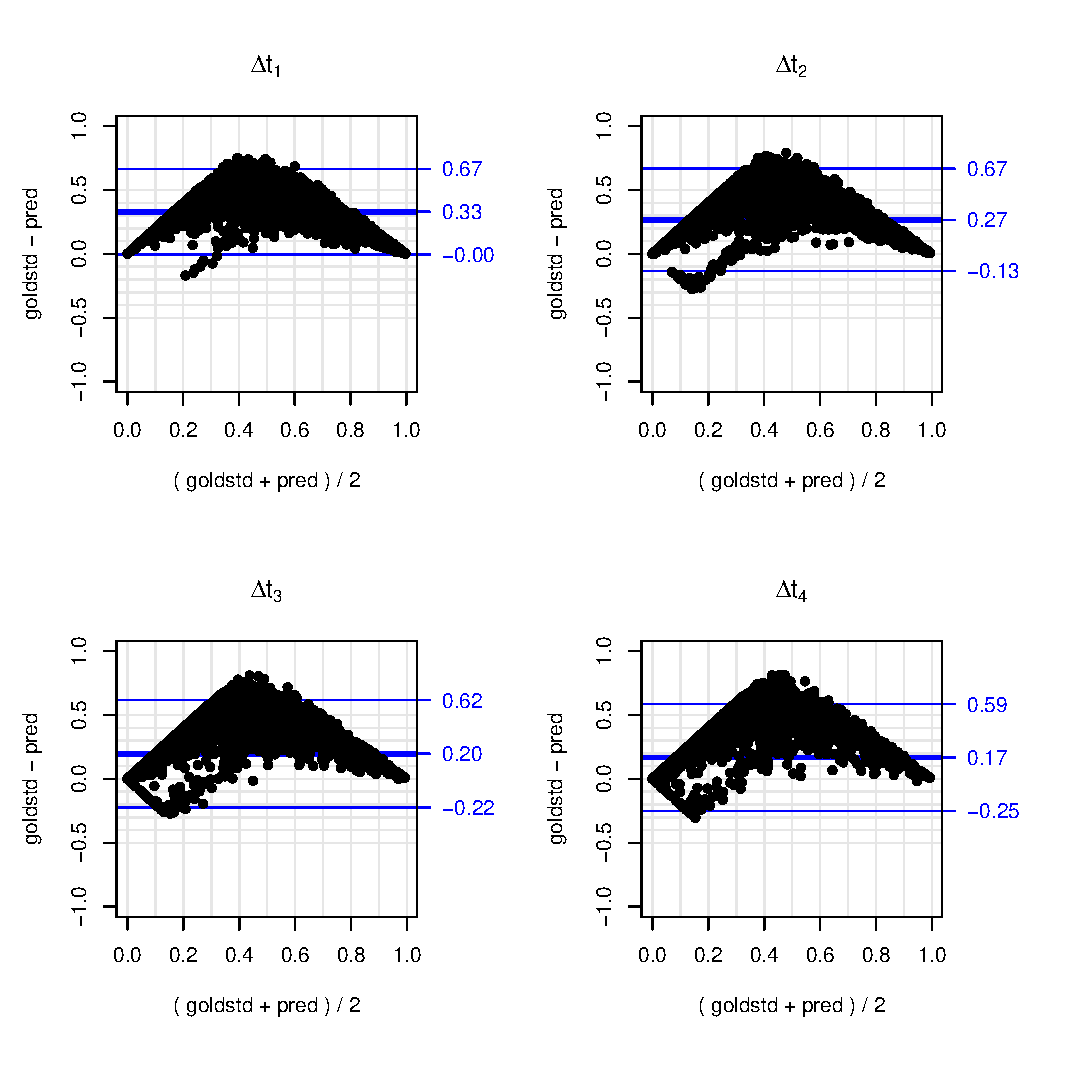
\includegraphics[width=0.45\columnwidth]{figures/baplot_qt25data_qt50fit_t1.eps}\label{plot:sim2fig12}
}

\subfloat[][LMJM]{
    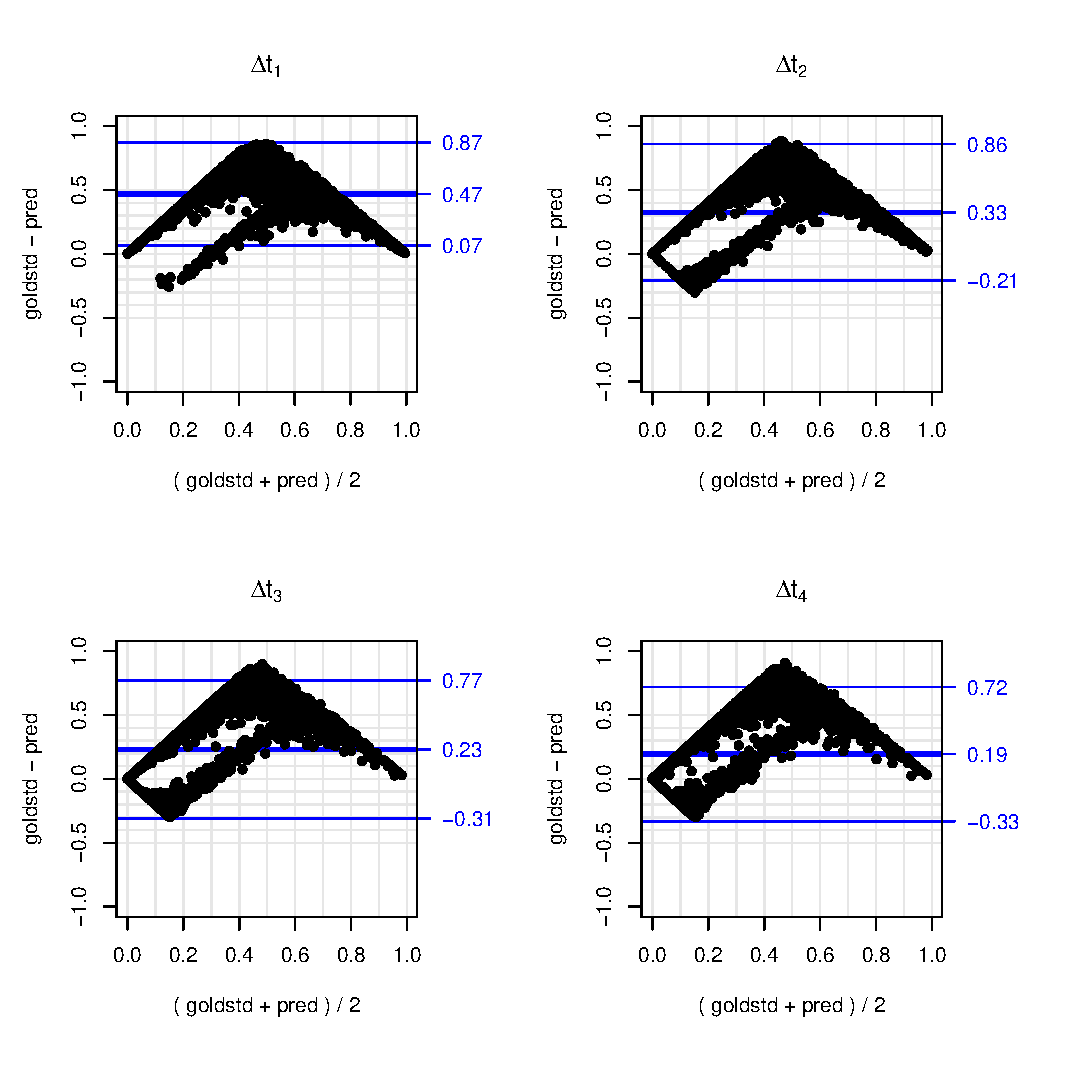
\includegraphics[width=0.45\columnwidth]{figures/baplot_qt25data_LMJMfit_t1.eps}\label{plot:sim2fig13}
}
  \caption{Prediction results in Simulation II Scenario 1: Bland-Altman plot (bias and 95\% limits of agreement) of gold standard versus model predictions at $t=0.25$ for four prediction time intervals ($\Delta t_1 < \Delta t_2 < \Delta t_3 < \Delta t_4$).}
  \label{plot:sim2fig1}
\end{figure}


\begin{figure}[H]
\centering
\subfloat[][LMJM (True model)]{
    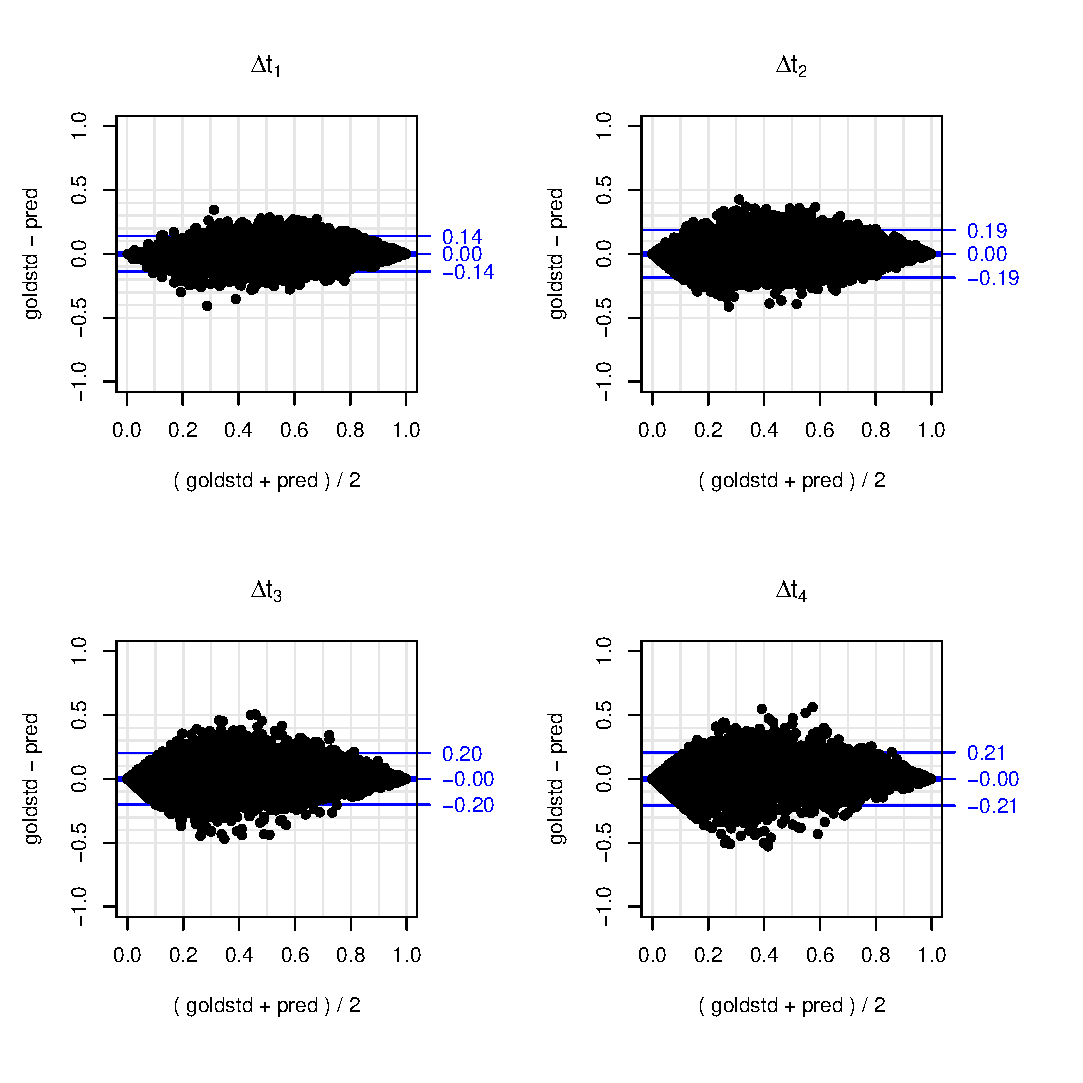
\includegraphics[width=0.45\columnwidth]{figures/baplot_normdata_LMJMfit_t1.eps}\label{fig:3a}
}
% \centering
\subfloat[][QRJM with $\tau=0.5$]{
    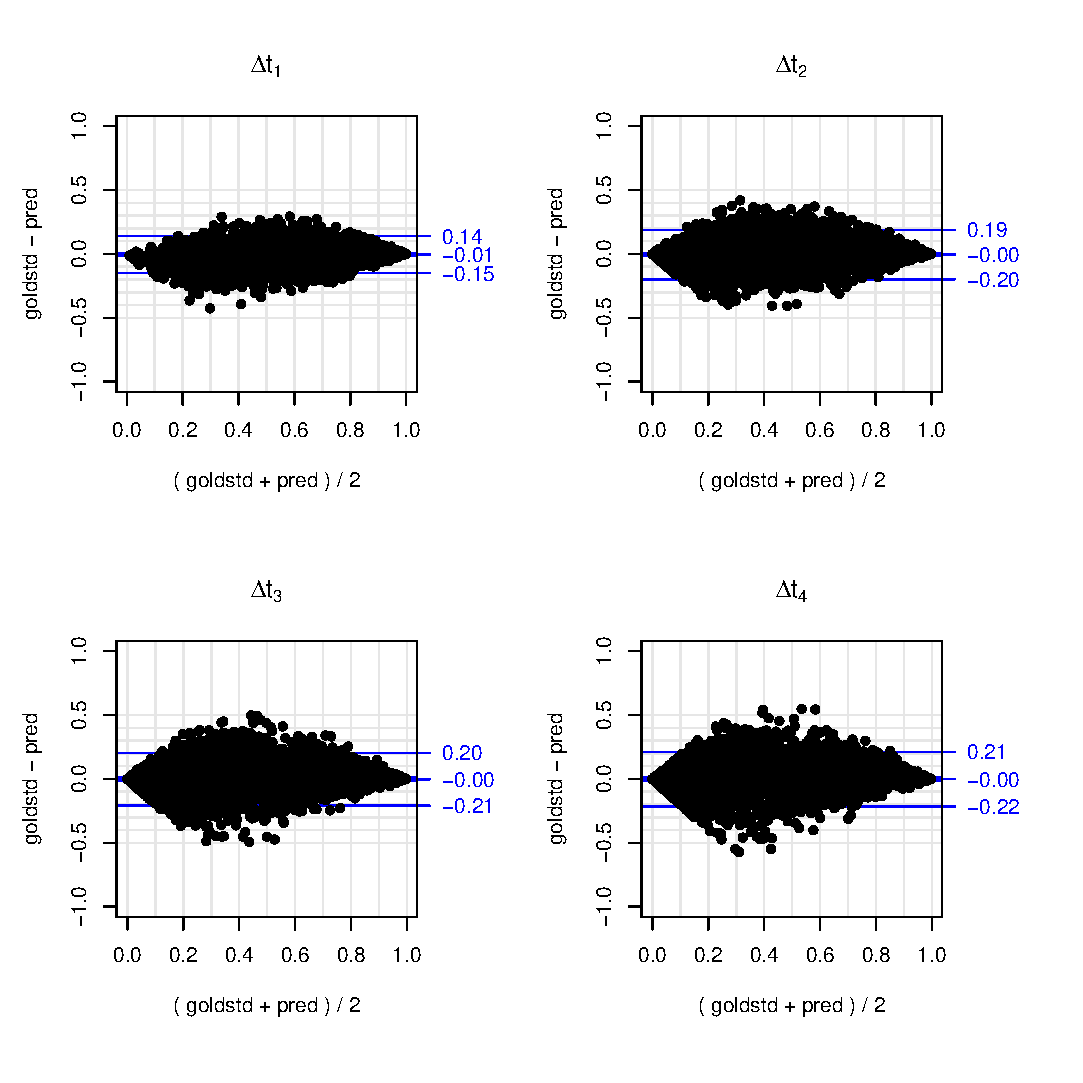
\includegraphics[width=0.45\columnwidth]{figures/baplot_normdata_qt50fit_t1.eps}\label{fig:3b}
}
  \caption{Prediction results in Simulation II Scenario 3: Bland-Altman plot (bias and 95\% limits of agreement) of gold standard versus model predictions at $t=0.25$ for four different prediction time intervals ($\Delta t_1 < \Delta t_2 < \Delta t_3 < \Delta t_4$).}
  \label{plot:sim2fig2}
\end{figure}


\newpage
\section{\textsf{JAGS} code to fit the QRJM in simulation study}
{\scriptsize
\begin{verbatim}
model{
  k1 <- (1-2*qt)/(qt*(1-qt))
  k2 <- 2/(qt*(1-qt))
  for (i in 1:I){
      # prior for random effects
      u[i, 1:2] ~ dmnorm(zero[], precision[,])
      # longitudinal process
      for (j in 1:J[i]){
          er[i,j] ~ dexp(sigma)
          mu[i,j] <- beta + u[i,1] + u[i,2]*t[j] + time[1]*X[i,1]
                    + time[2]*X[i,2]*t[j] + k1*er[i,j]
          prec[i,j] <- sigma/(k2*er[i,j])
          y[i,j] ~ dnorm(mu[i,j], prec[i,j])
      } #end of j loop
      # time-to-event process
      A[i] <- assoct.*u[i,2] + assoct.*time[2]*X[i,2]
      B[i] <- assoct.*(time[1]*X[i,1] + u[i,1] + beta) + inprod(gamma, W[i,])
      S[i] <- exp(-c*exp(B[i])*(exp(A[i]*Ti[i])-1)/A[i])
      h[i] <- c*exp(inprod(gamma, W[i,]) + assoct.*(beta +
            time[1]*X[i,1] + time[2]*X[i,2]*Ti[i] + u[i,1] + u[i,2]*Ti[i]))
      L[i] <- pow(h[i], event[i])*S[i]/1E+08
      phi[i] <- -log(L[i])
      zeros[i] ~ dpois(phi[i])
  }#end of i loop
  precision[1:2, 1:2] ~ dwish(Omega[,], 3)
  Sigma[1:2,1:2] <- inverse(precision[,])
  Omega[1,1] <- 1
  Omega[2,2] <- 1
  Omega[1,2] <- 0
  Omega[2,1] <- 0
  # priors for other parameters
  assoct. ~ dnorm(0, 0.001)
  int. ~ dnorm(0, 0.001)
  time[1] ~ dnorm(0, 0.001)
  time[2] ~ dnorm(0, 0.001)
  gamma[1] ~ dnorm(0, 0.001)
  gamma[2] ~ dnorm(0, 0.001)
  sigma ~ dgamma(0.001, 0.001)
  c ~ dunif(0.01, 10)
}
\end{verbatim}
}


\end{document}



